\documentclass[11pt,a4paper]{article}

\usepackage[utf8]{inputenc} 
\usepackage[T1]{fontenc} 
\usepackage{lmodern}
\usepackage[margin=2cm]{geometry}
\usepackage[german]{babel}
\usepackage{array}
\setlength{\parindent}{0pt}
\setlength{\parskip}{1ex plus 0.5ex minus 0.5ex}
\usepackage{amsmath} 
\usepackage{graphicx} 
\usepackage{booktabs}
\usepackage[colorlinks]{hyperref}
\usepackage{nicefrac}
\usepackage{gensymb}
\usepackage[usenames,dvipsnames,svgnames,table]{xcolor}
\usepackage{tcolorbox}
\usepackage[section]{placeins}

\hbadness=99999

\newenvironment{supbox}{\begin{tcolorbox}[colback=white,colframe=black,sharp corners,boxrule=.5pt]}{\end{tcolorbox}}
\begin{document}

{
\centering 
\large 
Physiklabor für Anf\"anger*innen \\
Ferienpraktikum im Sommersemester 2018 \\[4mm]
\textbf{\LARGE 
Versuch 31: Mischungsmethode in der Kalorimetrie
} \\[3mm]
(durchgef\"uhrt am 12.09.2018 bei Nico Strauß) \\
Andréz Gockel, Patrick M\"unnich\\
\today \\[10mm]
}

\section{Ziel des Versuchs}


Der Versuch ist in zwei Teile geteilt, welche dazu dienen, mit Hilfe einer geeigneten Wärmeenergiebilanz die Wärmekapazität zu bestimmen. Im Teil A kalibriert man das Messgerät und bestimmt mittels extrapolationsverfahren die Wärmekapazität des Kalorimeters. Für die Messungen wurde ein Temperaturmessfühler, der durch einen DAQ zu einem Komputer verbunden wurde verwendet, dadurch konnten die Messdaten mittels dem Programm LabVIEW gespeichert werden. Im Teil B wurde die Wärmekapazität von zwei Festkörpern bestimmt. 

\section{Auswertung und Fehleranalyse}

\subsection{Teil A - Kalibrierung des Messf\"uhlers}

\subsubsection{Aufgabenstellung}

Das Messprogramm, LabVIEW, soll vervollst\"andigt werden und der Messf\"uhler kalibriert.

\begin{figure}[ht!]
	\centering
	\fbox{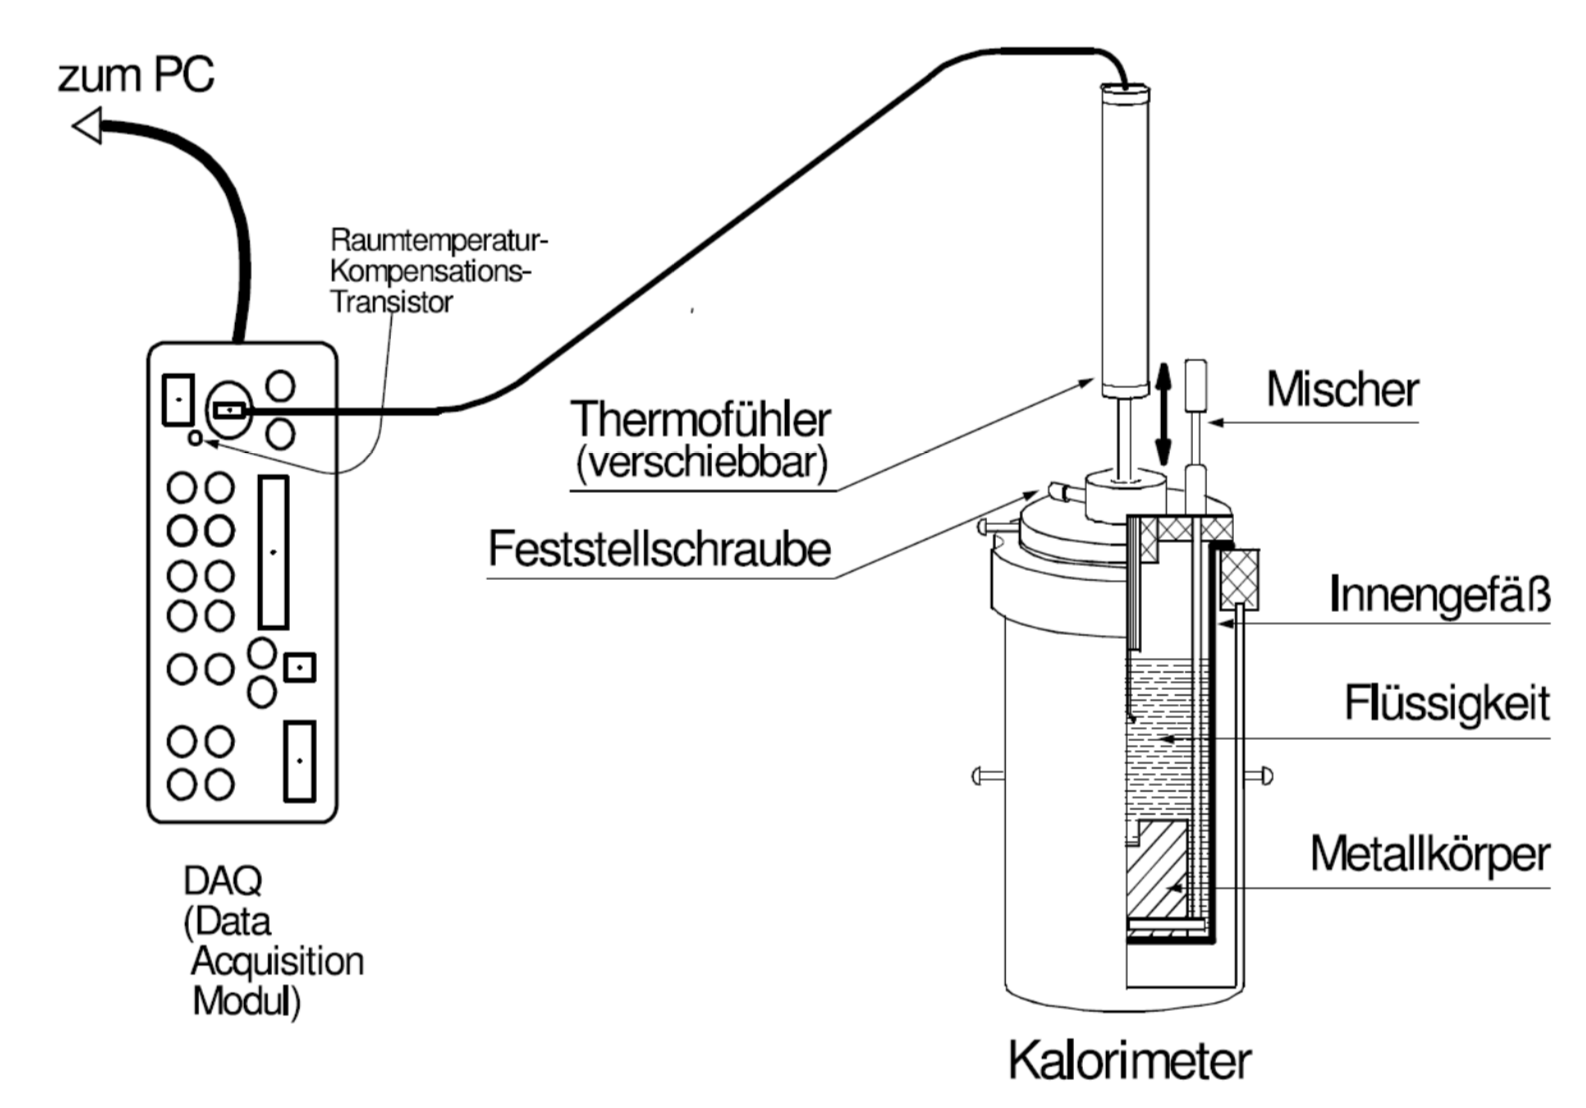
\includegraphics[width=0.7\textwidth]{Aufbaoo}}
  	\renewcommand\thefigure{B1}
	\caption{Der Aufbau}
	\label{Bild:1}
\end{figure}

\subsubsection{Ergebnisse}

Zur kalibrierung haben wir die Temperatur von Eiswasser und kochendem Wasser gemessen.

Nach der vervollst\"andigung des Programms wurden die Temperaturen von kochendem Wasser und Eiswasser gemessen. Diese wurden so angepasst, dass sie jeweils circa $100\celsius$ und $0\celsius$ waren. Gro\ss e Schwankungen waren jedoch auff\"allig. Bei dem kochenden Wasser waren diese eher klein, bei etwa $0.5\celsius$. Bei dem Eiswasser waren Schwankungen von $2\celsius$ zu beobachten, vermutlich aufgrund dem Aufw\"armen des Wassers. Man sollte also bei den folgenden Messungen die Temperaturen kurz vor dem Mischen messen, da diese sich leicht \"andern k\"onnen.

\subsection{Teil B - Bestimmung von der Wärmekapazität des Kalorimeters: $C_{kal}$}

\subsubsection{Aufgabenstellung}

Mithilfe der Mischungsmethode ist die W\"armekapazit\"at des Kalorimeters zu bestimmen. In diesem experiment wurden die Zeiten, Temperaturen und Massen gemessen.


%\subsubsection{Auswertung}
%\begin{table}
%\centering
%$\begin{array}{lr}
%	\multicolumn{2}{l}{\textrm{Messwerte zur Bestimmung von }C_{kal}}\\
%	\hline
%	\textrm{Wasser Masse} & 0\,\textrm{g} \\
%	\textrm{Temperatur Wasser 1} & 0\,\celsius \\
%	\textrm{Temperatur Wasser 2} & 100\,\celsius \\
%	\textrm{Temperatur nach Mischen} & 50\,\celsius\\
%	\hline
%\end{array}$
%\renewcommand\thetable{T1}
%\caption{Messwerte für Teil A}
%\label{tab:1}
%\end{table}

Zur bestimmung von $C_{kal}$ benutzen wir die Extrapolationsfunktionen (\ref{Bild:2}) und bestimmen daraus die Mischtemperatur. Die Funktion für das heiße Wasser wird mit $f_H$ bezeichnet, das kalte Wasser mit $f_K$ und für die Temperaturänderung während der Mischung mit $f_M$: 
$$f_H = -0.1305 t + 79.1561, \quad f_M = 4.049 + 20.866e^{-0.192t}, \quad f_K = -0.01288 t + 47.0561$$
Die Schnittstelle von $f_H$ und $f_M$ ist $t_1 = -2.7630$. Die Schnittstelle von $f_M$ und $f_K$ ist $t_2 = 10.3248$.
$$\int\displaylimits_{t_{ges}}^{t_2} f_M\ \mathrm{d}t - \int\displaylimits_{t_{ges}}^{t_2} f_K\ \mathrm{d}t = \int\displaylimits_{t_1}^{t_{ges}} f_H\ \mathrm{d}t - \int\displaylimits_{t_1}^{t_{ges}} f_M\ \mathrm{d}t$$ 
Aus dieser Gleichung wird die gesuchte Zeit $t_{ges}$ bestimmt und in $f_M$ eingesetzt. Der berechnete wert ist $t_{ges} = 36.8598$ (\ref{Bild:3}) 
$$4.049 + 20.866e^{-0.192\times 36.8598} = 44.07$$
Dieser wert wird als die Mischtemperatur $T_M$ verwendet. Für die spezifische Wärmekapazität von Wasser verwenden wir $c_W = 4.182$\,$\nicefrac{\mathrm{kJ}}{\textrm{kgK}}$. Mit der Formel 
\begin{equation}\label{E:1}
  C_{kal} = c_W(m_k\beta - m_h), \quad \beta = \frac{T_M - T_K}{T_H - T_M}
\end{equation}

Wobei die masse des kalten Wassers $m_k = 50.44(5)$\,g ist und die Masse des heißen Wassers $m_h = 103.59(5)$\,g ist.
Mit diesen Werten ergibt die Formel \ref{E:1} den wert $C_{kal} = $ für die Wärmekapazität des Kalorimeters.


\begin{figure}[h]
	\centering
	\fbox{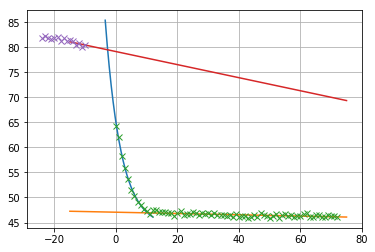
\includegraphics[width=0.5\textwidth]{Gmix}}
  	\renewcommand\thefigure{B2}
	\caption{Extrapolation}
	\label{Bild:2}
\end{figure}

\begin{figure}[p]
	\centering
	\fbox{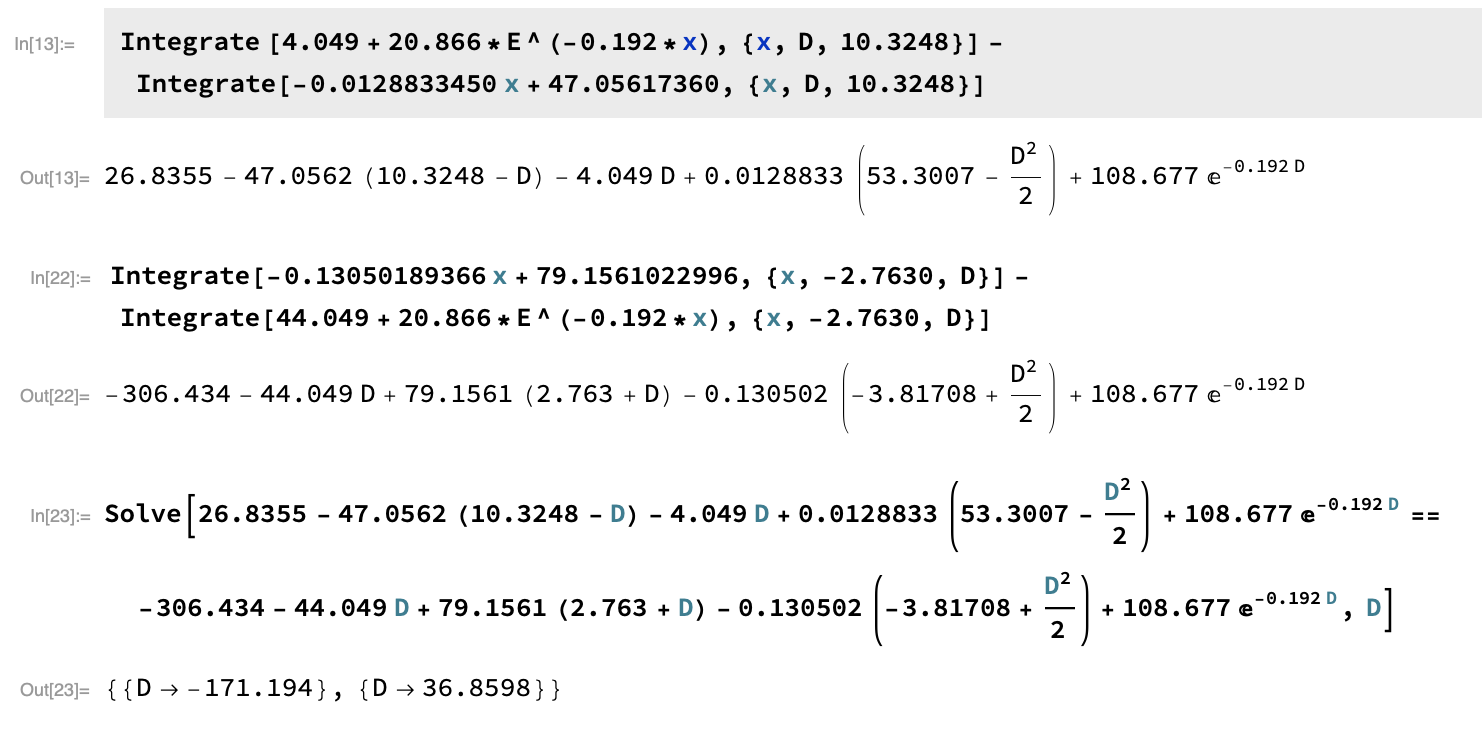
\includegraphics[width=0.7\textwidth]{RechKal}}
  	\renewcommand\thefigure{B3}
	\caption{Rechnung mit Mathematica}
	\label{Bild:3}
\end{figure}

\begin{supbox}
Es wurden zwei Messungen durchgef\"uhrt mit jeweils $116.94\,$g und $113.42\,$g Wasser. Die Wassermenge wurde so gew\"ahlt, damit der Widerstand und das Thermometer in dem Wasser eingetaucht sind. Die Dauern der Messungen waren 38 und 20 Minuten. Diese wurden so gew\"ahlt, dass sie m\"oglichst kurz ausfallen sollten. Temperatur\"anderungen wurden im Abstand von 60 Sekunden gemessen, da diese sonst nicht auff\"allig genug w\"aren, um etwas zu erkennen. Die Messwerte hierzu sind aufgrund ihrer L\"ange im Anhang.

Das extrapolationsverfahren der 1. Messreihe ergibt $T_{max} = 26.5\celsius$ da der Temperaturabfall erst nach 30 begann. Für die 2. Messreihe ergibt das extrapolationsverfahren $T_{max} = 41.45\celsius$ \ref{Dia:1}, \ref{Ext}
\end{supbox}
\begin{table}[h!]
	\centering
	\rowcolors{2}{gray!10}{white}
	\begin{tabular}{|c|cccc|}
		\multicolumn{5}{c}{\textrm{Extrapolationverfahren}} \\
		\noalign{\global\arrayrulewidth=0.4mm}
		\hline
		\noalign{\global\arrayrulewidth=0.2mm}
		\textrm{Messreihe} & $a$ in \celsius & $u_a$ in \celsius & b in $\nicefrac{\celsius}{\textrm{s}}$ & $u_b$ in $\nicefrac{\celsius}{\textrm{s}}$ \\
		\hline
	1 & 26.5 & 0.037 &  -33.579 & 2.105 $\times 10^{-5}$ \\
	2 & 42.65 & 1.605 & -0.0025 & 0.001443 \\
		\hline
	\end{tabular}
	\renewcommand\thetable{T3}
	\caption{Wertetablle für die extrapolation}
	\label{Ext}
\end{table}




%Systematische und statistische Fehler.


\subsection{Teil C - Bestimmung von der Spezifischen W\"armekapazit\"at von Festk\"orpern}

\subsubsection{Aufgabenstellung}

Ein Festk\"orper soll in einem Wasserbad erhitzt und anschlie\ss end in eine Fl\"ussigkeit im Kalorimeter gesteckt werden. Hierbei sollen die Massen, Temperaturen und Zeiten festgehalten werden, damit die W\"armekapazit\"at berechnet werden kann. Nach erfolgreicher Messung und Auswertung soll das Ergebniss mit dem Dulong-Petit-Gesetz verglichen werden.

\subsubsection{Auswertung}


\section{Anhang}

%\begin{figure}[p]
%\centering
%\fbox{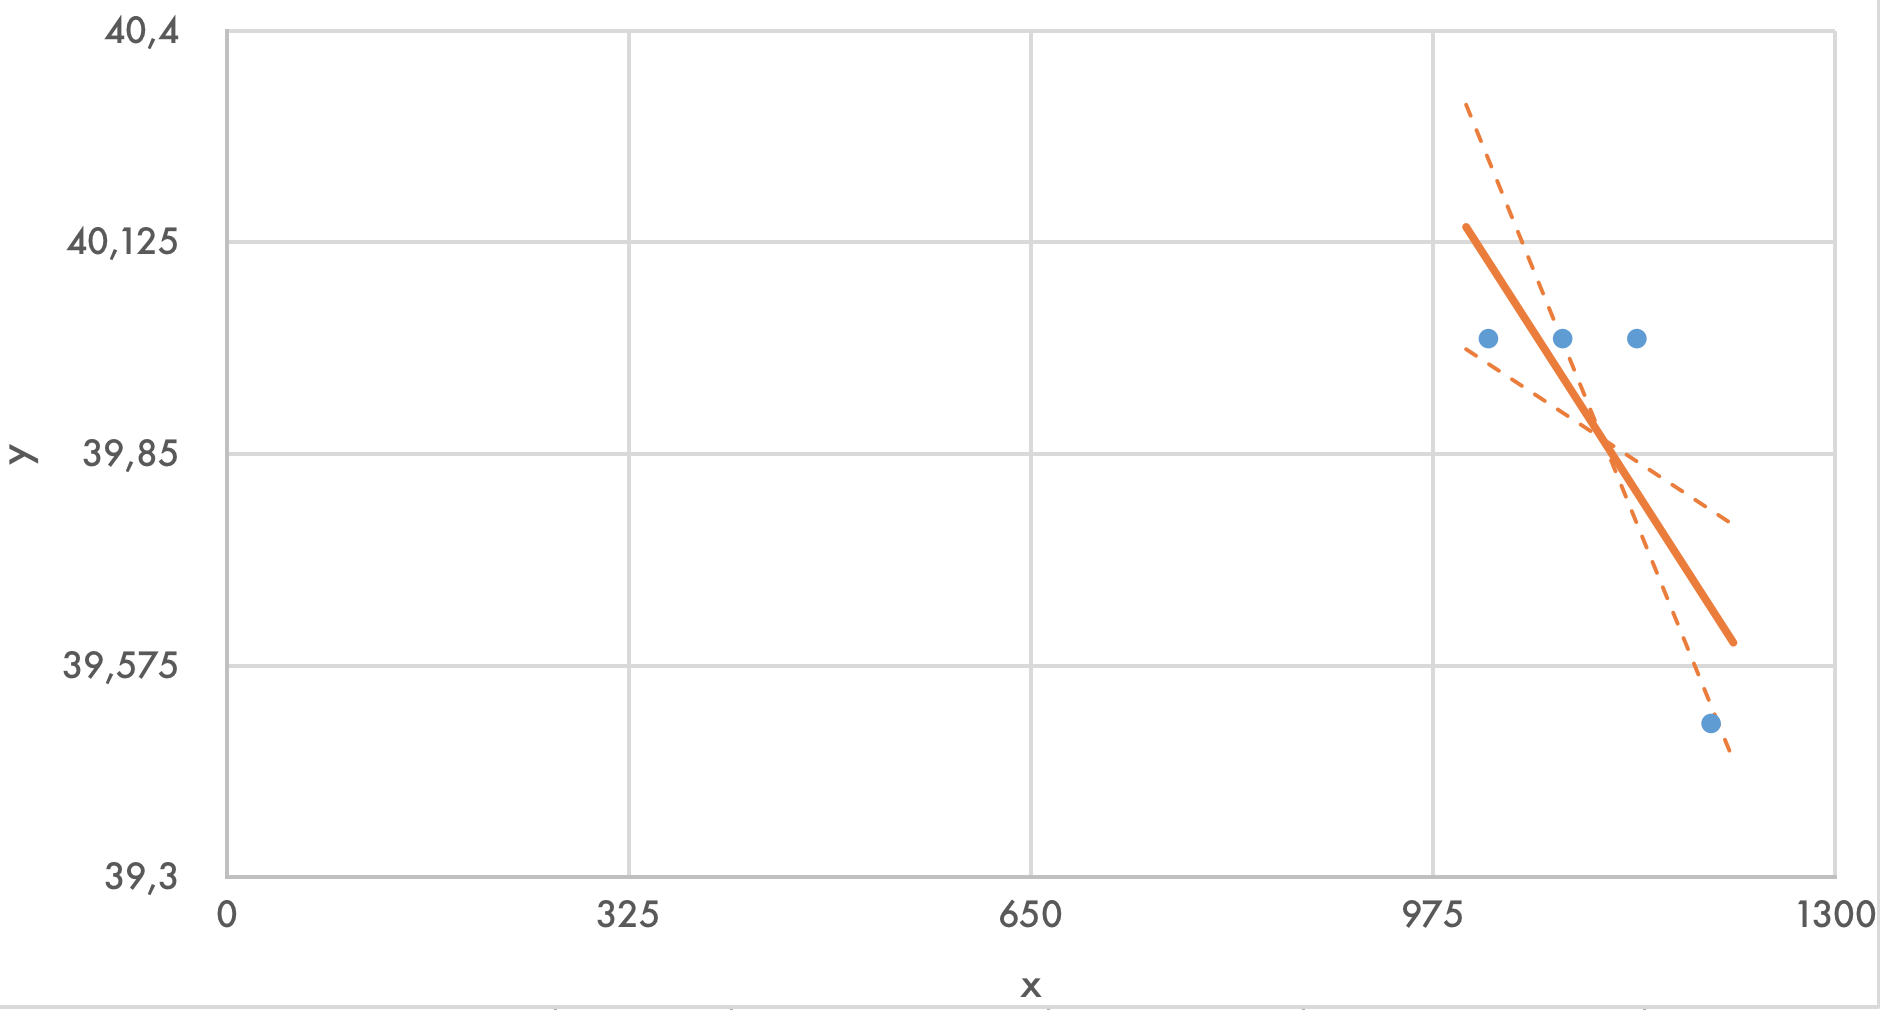
\includegraphics[width=0.7\textwidth]{extrapDia}}
%   \renewcommand\thefigure{A1}
%\caption{Extrapolation 2. Messreihe}
%\label{Dia:1}
%\end{figure}
%
%
%\begin{table}[p]
%	\centering
%	\rowcolors{2}{gray!10}{white}
%	\begin{tabular}{|r|l|}
%		\multicolumn{2}{c}{\textrm{Messreihe 1}} \\
%		\noalign{\global\arrayrulewidth=0.4mm}
%		\hline
%		\noalign{\global\arrayrulewidth=0.2mm}
%		\textrm{Rotationen }$n \pm 0.3$ & \textrm{Temperatur }$T \pm 0.05\celsius$\\
%		\hline
%		0 & 24 \\
%		10 & 24.1 \\
%		20 & 24.3 \\
%		30 & 24.5 \\
%		40 & 24.6 \\
%		50 & 24.8 \\
%		\hline
%	\end{tabular}
%	\renewcommand\thetable{T1}
%	\caption{Messreihe 1 für den ersten Versuchsteil}
%	\label{table:m1}
%\end{table}
%
%\begin{table}[p]
%	\centering
%	\rowcolors{2}{gray!10}{white}
%	\begin{tabular}{|r|l|}
%		\multicolumn{2}{c}{\textrm{Messreihe 2}} \\
%		\noalign{\global\arrayrulewidth=0.4mm}
%		\hline
%		\noalign{\global\arrayrulewidth=0.2mm}
%		\textrm{Rotationen }$n \pm 0.3$ & \textrm{Temperatur }$T \pm 0.05\celsius$\\
%		\hline
%		0 & 24.3 \\
%		5 & 24.3 \\
%		10 & 24.4 \\
%		15 & 24.5 \\
%		20 & 24.6 \\
%		25 & 24.7 \\
%		30 & 24.8 \\
%		35 & 24.9 \\
%		40 & 25 \\
%		45 & 25.1 \\
%		50 & 25.2 \\
%		55 & 25.2 \\
%		60 & 25.4 \\
%		65 & 25.5 \\
%		70 & 25.5 \\
%		75 & 25.6 \\
%		80 & 25.6 \\
%		85 & 25.7 \\
%		90 & 25.8 \\
%		95 & 26 \\
%		100 & 26 \\
%		\hline
%	\end{tabular}
%	\renewcommand\thetable{T2}
%	\caption{Messreihe 2 für den ersten Versuchsteil}
%	\label{table:m2}
%\end{table}
%
%\begin{table}[p]
%\centering
%$\begin{array}{rl}
%\multicolumn{2}{c}{\textrm{\underline{Unsicherheiten:}}}\\
%\textrm{Zeit: } & \pm 0.03 \textrm{s}\\
%\textrm{Temperatur: } & \pm 0.02 \textrm{\celsius}\\
%\textrm{Strom: } & \pm 0.03 \textrm{A}\\
%\textrm{Spannung: } & \pm 0.02 \textrm{V}
%\end{array}$
%\rowcolors{2}{gray!10}{white}
%\begin{tabular}{|c|c|c|c|}
%\multicolumn{4}{l}{Wasser 116.94(3)\,g}\\
%\hline
%$t$ in s & $T$ in $^\circ\textrm{C}$ & $I$ in A & $U$ in V \\
%\hline 
%0   & 22   & 1.5 & 14.9 \\
%60  & 22   & 1.5 & 14.9 \\
%120 & 23   & 1.5 & 14.9 \\
%180 & 24.5 & 0   & 0    \\
%240 & 26.3 & 0   & 0    \\ 
%300 & 26.5 & 0   & 0    \\ 
%360 & 26.5 & 0   & 0	\\ 
%$\vdots$ & $\vdots$ & $\vdots$ & $\vdots$ \\
%2280 & 26.4 & 0 & 0 \\
%\hline
%\end{tabular}
%\phantom{$\begin{array}{rl}
%\multicolumn{2}{l}{\textrm{\underline{Unsicherheiten:}}}\\
%\textrm{Zeit: } & \pm 0.03 \textrm{s}\\
%\textrm{Temperatur: } & \pm 0.02 \textrm{\celsius}\\
%\textrm{Strom: } & \pm 0.03 \textrm{A}\\
%\textrm{Spannung: } & \pm 0.02 \textrm{V}
%\end{array}$
%}
%\renewcommand\thetable{T4}
%\caption{1. Messwerte für Teil B}
%\label{tab:B1}
%\end{table}
%
%\begin{table}[p]
%\centering
%$\begin{array}{rl}
%\multicolumn{2}{l}{\textrm{\underline{Unsicherheiten:}}}\\
%\textrm{Zeit: } & \pm 0.03 \textrm{s}\\
%\textrm{Temperatur: } & \pm 0.02 \textrm{\celsius}\\
%\textrm{Strom: } & \pm 0.03 \textrm{A}\\
%\textrm{Spannung: } & \pm 0.02 \textrm{V}
%\end{array}$
%\rowcolors{2}{gray!10}{white}
%\begin{tabular}{|c|c|c|c|}
%\multicolumn{4}{l}{Wasser 113.42(3)\,g}\\
%\hline
%$t$ in s & $T$ in $^\circ\textrm{C}$ & $I$ in A & $U$ in V \\
%\hline 
%0   & 22 & 1.5 & 14.9\\
%60  & 22 & 1.5 & 14.9\\
%120 & 23 & 1.5 & 14.9\\
%180 & 24 & 1.5 & 14.9\\
%240 & 26 & 1.5 & 14.9\\ 
%300 & 27 & 1.5 & 14.9\\ 
%360 & 28 & 1.5 & 14.9\\ 
%420 & 29.2 & 1.5 & 14.9\\ 
%480 & 30.3 & 1.5 & 14.9\\ 
%540 & 31.9 & 1.5 & 14.9\\ 
%600 & 33 & 1.5 & 14.9\\ 
%660 & 33.7 & 1.5 & 14.9\\ 
%720 & 35 & 1.5 & 14.9\\ 
%780 & 35 & 1.5 & 14.9\\ 
%840 & 36 & 1.5 &14.9\\
%900 & 37 & 1.5 & 14.9\\
%960 & 38.2 & 0 & 0\\
%1020 & 39.5 & 0 & 0\\
%1080 & 40 & 0 & 0\\
%1140 & 40 & 0 & 0\\
%1200 & 39.5 & 0 & 0\\
%\hline
%\end{tabular}
%\phantom{$\begin{array}{rl}
%\multicolumn{2}{l}{\textrm{\underline{Unsicherheiten:}}}\\
%\textrm{Zeit: } & \pm 0.03 \textrm{s}\\
%\textrm{Temperatur: } & \pm 0.02 \textrm{\celsius}\\
%\textrm{Strom: } & \pm 0.03 \textrm{A}\\
%\textrm{Spannung: } & \pm 0.02 \textrm{V}
%\end{array}$
%}
%\renewcommand\thetable{T5}
%\caption{2. Messwerte für Teil B}
%\label{tab:B2}
%\end{table}


\end{document}